\documentclass{article}

\usepackage{graphicx}
\usepackage{rotating}
\usepackage{amsmath}
\usepackage{amssymb}
\usepackage{mathrsfs}
\usepackage{fancyhdr}
\usepackage{listings}
\usepackage{xcolor}
\usepackage{color}
\usepackage{amsfonts}
\usepackage{textcomp}
\usepackage{float}
\usepackage{neuralnetwork}
\usepackage{pgfplots}
\usepackage[sorting=none]{biblatex}
\usepackage[margin=1in]{geometry}
\usepackage[font={small,it}]{caption}
\usepackage{placeins}
\usepackage{xepersian}

\pgfplotsset{width=8cm,compat=1.17}

%\DeclareMathOperator*{\btie}{\bowtie}
\addbibresource{bibliography.bib}
\settextfont[Scale=1.2]{B-NAZANIN.TTF}
\setlatintextfont[Scale=1]{Times New Roman}
\renewcommand{\baselinestretch}{1.5}
\pagestyle{fancy}
\fancyhf{}
\rhead{تکلیف دوم درس یادگیری عمیق}
\lhead{\thepage}
\rfoot{علیرضا ابره فروش}
\lfoot{9816603}
\renewcommand{\headrulewidth}{1pt}
\renewcommand{\footrulewidth}{1pt}
\newcommand{\Lagr}{\mathcal{L}}
\newcommand{\Mod}[1]{\ (\mathrm{mod}\ #1)}
%%%%%%%%%%
\lstset
{
    language=[latex]tex,
    basicstyle=\ttfamily,
    commentstyle=\color{black},
    columns=fullflexible,
    keepspaces=true,
    upquote=true,
    showstringspaces=false,
    morestring=[s]\\\%,
    stringstyle=\color{black},
}
%%%%%%%%%%
%beginMatlab
\definecolor{mygreen}{RGB}{28,172,0} % color values Red, Green, Blue
\definecolor{mylilas}{RGB}{170,55,241}
%endMatlab
\begin{document}
%beginMatlab
\lstset{language=Matlab,%
    %basicstyle=\color{red},
    breaklines=true,%
    morekeywords={matlab2tikz},
    keywordstyle=\color{blue},%
    morekeywords=[2]{1}, keywordstyle=[2]{\color{black}},
    identifierstyle=\color{black},%
    stringstyle=\color{mylilas},
    commentstyle=\color{mygreen},%
    showstringspaces=false,%without this there will be a symbol in the places where there is a space
    numbers=left,%
    numberstyle={\tiny \color{black}},% size of the numbers
    numbersep=9pt, % this defines how far the numbers are from the text
    emph=[1]{for,end,break},emphstyle=[1]\color{red}, %some words to emphasise
    %emph=[2]{word1,word2}, emphstyle=[2]{style},    
}
%endMatlab
\begin{titlepage}
\begin{center}
\includegraphics[width=0.4\textwidth]{IUT Logo.png}\\
        
\LARGE
\textbf{دانشگاه صنعتی اصفهان}\\
\textbf{دانشکده مهندسی برق و کامپیوتر}\\
        
\vfill
        
\huge
\textbf{عنوان: تکلیف اول درس سیستم‌های عامل 1}\\
        
\vfill
        
\LARGE
\textbf{نام و نام خانوادگی: علیرضا ابره فروش}\\
\textbf{شماره دانشجویی: 9816603}\\
\textbf{نیم\,سال تحصیلی: پاییز 1400}\\
\textbf{مدرّس: دکتر محمّدرضا حیدرپور}\\
\textbf{دستیاران آموزشی: مجید فرهادی - دانیال مهرآیین - محمّد نعیمی}\\
\end{center}
\end{titlepage}


%\tableofcontents
\newpage


%1
\section{}
\subsection{الف}

توابع فعال‌سازی واحد خطی تصحیح شده \lr{(ReLU)} به چند دلیل به طور معمول در یادگیری عمیق بیشتر از توابع فعال‌سازی تانژانت هایپربولیک (\lr{tanh}) مورد استفاده قرار می‌گیرند:
\begin{enumerate}
\item مشکل محو شیب: توابع فعال‌سازی تانژانتی این خاصیت را دارند که مشتق آن‌ها در اطراف مقدار 0 بیشترین مقدار را دارد. این به معنای آن است که در هنگام بازگشتی به عقب (\lr{backpropagation}) ، زمانی که شیب محاسبه و به عقب از طریق شبکه منتقل می‌شود، شیب‌ها به اندازه‌ای کوچک می‌شوند که با افزایش مقدار مطلق ورودی، بسیار کوچک می‌شوند. این می‌تواند به مشکل محو شیب \lr{(vanishing gradient)} منجر شود که در آن لایه‌های اولیه یک شبکه عمیق مقدار به‌روزرسانی کمی دریافت می‌کنند و به سختی می‌توانند به طور مؤثر یاد بگیرند. از طرف دیگر، تابع \lr{ReLU} این مشکل محو شیب را ندارد زیرا مشتق آن برای ورودی‌های مثبت 1 است.

\item محاسبه ساده‌تر: تابع \lr{ReLU} از نظر محاسباتی ارزان‌تر از تابع \lr{tanh} است. محاسبه تابع \lr{tanh} شامل توان‌گیری و تقسیم است، که عملیات محاسباتی مقایسه شده با عملیات آستانه‌گذاری ساده تابع \lr{ReLU} بیشتر توان مصرف می‌کند. این باعث می‌شود که \lr{ReLU} موثرتر و سریعتر برای آموزش باشد.

\item \lr{sparsity} و غیرخطیت: واحدهای \lr{ReLU} می‌توانند \lr{sparsity} در شبکه ایجاد کنند. زیرا برای ورودی‌های منفی خروجی 0 می‌دهند. \lr{sparsity} در برخی موارد مفید است. زیرا شبکه را تشویق می‌کند که بر روی زیرمجموعه‌ای از ویژگی‌های ورودی تمرکز کند. علاوه بر این، واحدهای \lr{ReLU} غیرخطیت ارائه می‌دهند که برای مدل کردن توابع پیچیده توسط شبکه‌های عمیق مورد نیاز است.

\item موفقیت تجربی: توابع \lr{ReLU} در آموزش شبکه‌های عصبی عمیق موفقیت نشان داده‌اند. آن‌ها به طور گسترده در معماری‌های مختلف یادگیری عمیق مانند شبکه‌های عصبی کانوولوشنی (\lr{CNN}) و شبکه‌های عصبی مکرر (\lr{RNN}) به کار رفته‌اند و در مدل‌های برتر متعددی استفاده شده‌اند.
\end{enumerate}

با این حال، مهم است به یاد داشت که تابع \lr{ReLU} همراه با محدودیت‌های خود نیز هست. ممکن است مشکل "مرگ \lr{ReLU}" رخ دهد که در آن واحدهای \lr{ReLU} طی آموزش غیرفعال شوند (همیشه خروجی 0 دهند) و هیچگاه به حالت عادی باز نگردند. این مشکل با استفاده از نسخه‌های تغییریافته از \lr{ReLU} مانند \lr{Leaky ReLU} یا \lr{Parametric ReLU} قابل حل است که به واحدها امکان می‌دهد که برای ورودی‌های منفی شیبی کوچک داشته باشند و جلوی غیرفعال شدن کامل واحدها را بگیرند.

در عمل، انتخاب بین \lr{ReLU} و \lr{tanh} به مسئله خاص، معماری شبکه و سایر پارامترهای مدل بستگی دارد. در این مورد پاسخ یکتایی وجود ندارد و پژوهشگران اغلب با توابع فعال‌سازی مختلف آزمایش می‌کنند تا بیابند کدام تابع برای یک وظیفه خاص بهتر عمل می‌کند.

\subsection{ب}
یکی از مهم‌ترین موانع در آموزش شبکه‌های عصبی عمیق (\lr{DNN})، مشکل محو شیب است که در آن شیب‌ها (گرادیان‌ها) تابع هزینه نسبت به وزن‌های لایه‌های اولیه به‌طور قابل‌توجهی کوچک می‌شوند. به عبارت دیگر، لایه‌های اولیه کمتر یا اصلاً اطلاعات وزن به‌روزشده‌ای در هنگام بازگشت به عقب (\lr{backpropagation}) دریافت می‌کنند که به همگرایی کند یا حتی رکود منتج می‌شود. مشکل محو شیب به‌طور اصلی به انتخاب توابع فعال‌ساز و روش‌های بهینه‌سازی در شبکه‌های عصبی عمیق مرتبط است.

روابط مشتق دو تابع به همراه نمودار مشتق آن‌ها رسم شده است.

\begin{latin}
\subsubsection{\lr{ReLU}}
$
ReLU(x) = x ^ + = \max(0, x)\\
ReLU'(x) =
\begin{cases}
0, & \text{if } x < 0 \\
1, & \text{if } x \geq 0
\end{cases}
$
\subsubsection{\lr{Sigmoid}}
$
\sigma(x) = \frac{1}{1 + e ^ {-x}} \\
\sigma'(x) = \sigma(x) \left( 1 - \sigma(x) \right)
$
%%%%%%%%%
\begin{figure}[htbp]
\centering
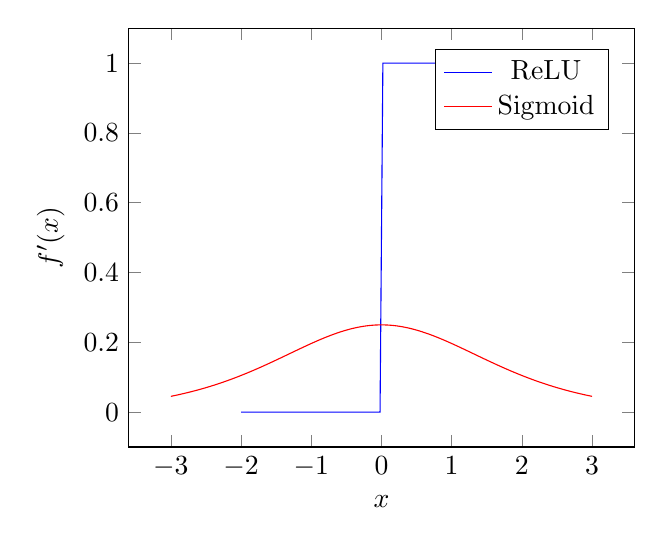
\begin{tikzpicture}
\begin{axis}[
    xlabel={$x$},
    ylabel={$f'(x)$},
    legend style={at={(0.95,0.95)},anchor=north east},
]

% ReLU derivative
\addplot[blue, domain=-2:2, samples=100] {x > 0 ? 1 : 0};
\addlegendentry{ReLU}

% Sigmoid derivative
\addplot[red, domain=-3:3, samples=100] {exp(-x)/(1+exp(-x))^2};
\addlegendentry{Sigmoid}

\end{axis}
\end{tikzpicture}
\caption{Derivatives of ReLU and Sigmoid functions.}
\end{figure}
%%%%%%%%%
\end{latin}


شیب توابع فعال‌ساز سیگمویدی به طور معمول به سرعت محو می‌شوند. یک بازه نسبتاً کوچکی از ورودی‌ها وجود دارد که مشتق تابع سیگموید به میزان کافی غیرصفر است. به عبارت دیگر، هنگامی که سیگموید به یکی از دو قله چپ یا راست می‌رسد، تقریباً بی‌معنی است که یک مرور به عقب از آن انجام داده شود، زیرا مشتق به صفر میل می‌کند. از سوی دیگر، تابع \lr{ReLU} تنها هنگامی اشباع می‌شود که ورودی کمتر از صفر باشد. حتی این اشباع می‌تواند با استفاده از واحدهای \lr{Leaky ReLU} مهار شود. در شبکه‌های عمیق، اشباع یادگیری را مختل می‌کند، بنابراین \lr{ReLU} می‌تواند راه‌حل مناسب‌تری نسبت به سیگموید باشد. البته باید به یاد داشت که با توجه به نوع داده و شرایط مسئله هر یک این توابع می‌تواند عملکرد بهتری نسبت به دیگری داشته باشد.
\subsection{ج}

وقتی مقدار اولیه وزن‌ها در یک شبکه عصبی با تابع فعال‌سازی \lr{Sigmoid} بسیار بزرگ باشد، چند مشکل ممکن است پیش بیاید:
\begin{enumerate}
\item    اشباع شبکه: ورودی‌های بزرگ باعث می‌شود تابع فعال‌سازی \lr{Sigmoid} به سرعت به 1 (یا به سمت صفر) اشباع شود. این به این معناست که توابع فعال‌سازی \lr{Sigmoid} به سرعت مقدار‌های خروجی نزدیک به 1 (یا 0) تولید می‌کنند، و این می‌تواند به مشکل شبکه اصلی شما بیافزاید، زیرا گرادیان‌ها به سرعت به صفر نزدیک می‌شوند.

\item    مشکل محو شیب: همچنین، وقتی مقدار وزن‌ها بسیار بزرگ باشد، مشکل محو شیب (\lr{vanishing gradient}) نیز ممکن است به وجود بیاید. زیرا مشتق تابع \lr{Sigmoid} در نزدیکی نقطه میانی (0.5) بیشینه می‌شود و با افزایش فاصله از این نقطه در هر دو جهت، مشتق به سرعت به صفر نزدیک می‌شود. این موجب می‌شود که گرادیان‌ها بسیار کوچک شوند و به شبکه کمکی در آموزش نکنند.

\item    سختی آموزش: شبکه‌های عصبی با تابع فعال‌سازی \lr{Sigmoid} و وزن‌های بزرگ ممکن است به سرعت به مسئله آموزش نشدنی تبدیل شوند. آموزش شبکه‌های ژرف با این ویژگی‌ها به طور کلی سخت‌تر است و نیازمند تنظیمات و حل مشکلات ویژه‌ای می‌باشد.
\end{enumerate}

برای مقابله با این مشکلات، می‌توان از مقادیر اولیه وزن مناسب‌تری استفاده کرد، مانند مقادیر تصادفی کوچکتر یا از روش‌های مانند نرمالیزه کردن وزن‌ها بهره برد. همچنین، ممکن است از توابع فعال‌سازی دیگری که بهتر با مقادیر بزرگ کار می‌کنند، مانند \lr{ReLU} یا \lr{Leaky ReLU}، استفاده کرد. انتخاب تابع فعال‌سازی و مقادیر اولیه وزن‌ها باید به توجه به کاربرد و معماری خاص شبکه انجام شود.


%2
\section{}
\subsection{الف}
در شبکه‌های عصبی، استفاده از توابع فعال‌ساز غیرخطی به دلایل متعددی ضروری است:
\begin{enumerate}
\item    قابلیت نمایش توابع پیچیده: توابع فعال‌ساز غیرخطی امکان نمایش توابع پیچیده‌تری را فراهم می‌کنند. اگر از توابع خطی استفاده شود (مثل تابع همانی)، شبکه توانایی نمایش توابع پیچیده و غیرخطی را نخواهد داشت. توابع غیرخطی می‌توانند الگوهای پیچیده‌تر و ساختارهای عمیق‌تر را مدل کنند.

\item    اهمیت انطباق به داده: توابع غیرخطی به شبکه‌های عصبی اجازه می‌دهند که بهتر به داده‌ها انطباق پیدا کنند. این به معنای این است که توابع فعال‌سازی غیرخطی می‌توانند بر اساس ویژگی‌های داده و نمونه‌ها، تغییر کنند و توانایی شبکه را در تطبیق بهتر با تغییرات در داده ارتقا می‌دهند.

\item    مدل‌سازی تعاملات غیرخطی: در بسیاری از کاربردها، ارتباطات و تعاملات بین متغیرها و ویژگی‌های ورودی غیرخطی هستند. توابع فعال‌سازی غیرخطی به شبکه‌ها امکان می‌دهند تا تعاملات غیرخطی را به خوبی مدل کنند و از توانایی شبکه در پیش‌بینی تعاملات پیچیده بهره‌برند.

\item    مشکل محو شیب را کاهش می‌دهند: توابع غیرخطی معمولاً مشکل محو شیب را کاهش می‌دهند. توابع خطی به سرعت به صفر همگرا می‌شوند و مشتق‌های کوچکی دارند، اما توابع فعال‌سازی غیرخطی (مانند \lr{ReLU}) مشتق‌های بزرگ‌تری دارند و این به شبکه‌ها امکان می‌دهد که در دوره‌های آموزشی عمیق‌تر پایدارتر باشند.
\end{enumerate}

با توجه به این دلایل، توابع فعال‌سازی غیرخطی مهمی در موفقیت شبکه‌های عصبی در مدل‌سازی و پیش‌بینی وظایف پیچیده و غیرخطی ایفا می‌کنند.

\subsection{ب}
\begin{latin}
$
g\left( x \right) = - \min\left( 5, x \right)\\
h\left( x \right) =
\begin{cases}
\max\left( x, 0.3x \right), & x \geq 0\\
\min\left( x, 0.3x \right), & x < 0
\end{cases} \\ \overset{\text{if } x \geq 0: \:\: x \geq 0.3x}{\underset{\text{if } x < 0: \:\: x < 0.3x}{\Longrightarrow }}
h\left( x \right) = x
$

\begin{figure}[htbp]
\centering
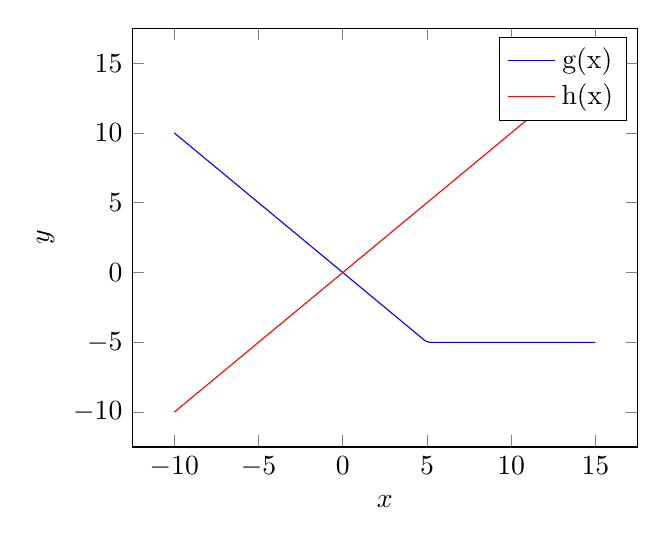
\begin{tikzpicture}
\begin{axis}[
    xlabel={$x$},
    ylabel={$y$},
]

% Plot of g(x) = -min(5, x) in blue
\addplot[blue, domain=-10:15, samples=100] {-min(5, x)};
\addlegendentry{g(x)}

% Plot of h(x) = x in red
\addplot[red, domain=-10:15, samples=100] {x};
\addlegendentry{h(x)}

\end{axis}
\end{tikzpicture}
\caption{Plot of $g(x) = -\min(5, x)$ and $h(x) = x$}
\end{figure}
\end{latin}
توابع فعال‌ساز نقش حیاتی در شبکه‌های عصبی عمیق دارند و تأثیر زیادی بر توانایی شبکه در یادگیری و حل مسائل مختلف دارند. انتخاب توابع فعال‌ساز می‌تواند به طور قابل توجهی بر آموزش و عملکرد شبکه تأثیر بگذارد.

\subsubsection{$g(x)$}

این تابع حداقل مقدار بین $x$ و 5 را می‌گیرد، آن را منفی می‌کند و نتیجه را به عنوان خروجی استفاده می‌کند. این تابع می‌تواند به عنوان تابع فعال‌سازی استفاده شود، اما مشکلاتی دارد:
\begin{enumerate}
\item    اشباع: این تابع برای مقادیر $x > 5$ صاف می‌شود و گرادیان آن در این ناحیه صفر است. این می‌تواند منجر به محو شدن گرادیان‌ها در هنگام \lr{backpropagation} شود، که باعث دشوار شدن آموزش شبکه می‌شود.

\item    عدم غیرخطیت: توابع فعال‌سازی باید غیرخطیت را به وارد شبکه کنند. $g(x)$ یک تابع قطعه قطعه خطی است که تنها یک نقطه انحراف در $x = 5$ دارد. این کمبود غیرخطیت می‌تواند توانایی شبکه در مدل کردن روابط پیچیده در داده‌ها را محدود کند.

\item    عدم محبوبیت: این تابع در عمل برای شبکه‌های عصبی عمیق به صورت معمول مورد استفاده قرار نمی‌گیرد، و توابع فعال‌سازی معتبرتری وجود دارند که به خوبی کار می‌کنند، مانند \lr{ReLU} و نسخه‌های مشتق شده از آن.

\end{enumerate}

\subsubsection{$h(x)$}

این تابع یک تابع فعال‌سازی خطی است، یعنی غیرخطیتی را به شبکه معرفی نمی‌کند. اگرچه ممکن است در برخی معماری‌های شبکه‌های عصبی (مانند رگرسیون خطی) مورد استفاده قرار گیرد، اما به طور کلی در شبکه‌های عصبی عمیق به عنوان تابع فعال‌سازی استفاده نمی‌شود، به علت دلایل متعددی از جمله:
\begin{enumerate}
\item    ظرفیت مدل‌سازی محدود: شبکه‌های عصبی عمیق از توابع فعال‌سازی غیرخطی برای مدل‌سازی روابط غیرخطی و پیچیده در داده‌ها استفاده می‌کنند. استفاده از $h(x) = x$ در تمام شبکه تقریباً شبیه به یک مدل خطی تک لایه می‌شود و توانایی نمایش الگوهای پیچیده را محدود می‌کند.
\end{enumerate}

%3
\section{}
\subsection{الف}
تابع تانژانت هایپربولیک ($tanh$) اغلب به عنوان نسخه مقیاس‌شده‌ای از تابع سیگموید توصیف می‌شود، به خصوص تابع سیگموید لجستیک. این رابطه به دلیل شباهت‌های تابع تانژانت و تابع سیگموید وجود دارد، اما در بازه و مقیاس‌شان تفاوت دارند.\\
تابع سیگموید که اغلب با نماد $\sigma\left( x \right)$ نشان داده می‌شود، به شرح زیر تعریف می‌شود:
\begin{latin}
$
\sigma\left( x \right) = \frac{1}{1 + e ^ {-x}}
$
\end{latin}
این تابع هر عدد حقیقی را به یک مقدار بین 0 و 1 نگاشت می‌کند. وقتی $x$ یک عدد مثبت بزرگ است، $\sigma\left( x \right)$ به 1 نزدیک می‌شود و وقتی $x$ یک عدد منفی بزرگ است، $\sigma\left( x \right)$ به 0 نزدیک می‌شود. این به این معناست که تابع سیگموید ورودی خود را در بازه (0، 1) فشرده می‌کند که برای مسائل دسته‌بندی دودویی مفید است، چون می‌توان از آن تعبیر احتمالاتی کرد.\\
تابع تانژانت هایپربولیک، به شکل زیر تعریف می‌شود:
\begin{latin}
$
tanh(x) = \frac{e^x - e^{-x}}{e^x + e^{-x}} = \frac{e ^ {2x} - 1}{e ^ {2x} + 1}
$
\end{latin}
تابع تانژانت هایپربولیک هر عدد حقیقی را به یک مقدار بین 1- و 1 نگاشت می‌دهد. وقتی $x$ یک عدد مثبت بزرگ است، $tanh(x)$ به 1 نزدیک می‌شود و وقتی $x$ یک عدد منفی بزرگ است، $tanh(x)$ به 1- نزدیک می‌شود.\\

رابطه بین توابع تانژانت هایپربولیک و سیگموید به شرح زیر است:
\begin{enumerate}
\item مقیاس‌دهی: تابع تانژانت هایپربولیک، انتقال داده شده و مقیاس شده‌ی تابع سیگموید به منظور داشتن رنج $(-1, 1)$ به جای $(0, 1)$ است. این مقیاس‌دهی با کم کردن $0.5$ از تابع سیگموید و سپس ضرب آن در 2 انجام می‌شود:
\begin{latin}
$
2\sigma\left( 2x \right)-1 = 
2 \times \frac{1}{1 + e ^ {-2x}} - 1 =
\frac{1 - e ^ {-2x}}{1 + e ^ {-2x}} = 
\frac{1 - e ^ {-2x}}{1 + e ^ {-2x}} \times \frac{e ^ {2x}}{e ^ {2x}} =
\frac{e ^ {2x} - 1}{e ^ {2x} + 1} = tanh\left( x \right)\\ \Rightarrow 
tanh(x) = 2\sigma\left( 2x \right) - 1
$
\end{latin}

\item تقارن: یکی از تفاوت‌های کلیدی این است که تابع تانژانت هایپربولیک در اطراف مبدأ متقارن است (در واقع $tanh(-x) = -tanh(x)$)، درحالی که تابع سیگموید این تقارن را ندارد.

\end{enumerate}
تابع تانژانت هایپربولیک اغلب به عنوان یک جایگزین برای تابع سیگموید در شبکه‌های عصبی استفاده می‌شود. زیرا به دلیل ماهیت مرکز شده حول صفری که دارد، یادگیری در شبکه‌های عمیق را سریع‌تر می‌کند. اینکه تابع تانژانت هایپربولیک مقادیر منفی را نیز خروجی دهد به معنای این است که می‌تواند تغییرات مثبت و منفی را در واحدهای مخفی شبکه در طول آموزش ایجاد کند که می‌تواند به همگرایی کمک کند. با این حال، هر دو تابع هنوز در متنوعی از زمینه‌ها استفاده می‌شوند و انتخاب بین آن‌ها بستگی به مسئله خاص و معماری شبکه دارد.



\subsection{ب}
\begin{latin}
$
p\left( x \right) = x \log\left( 1 + tanh\left( e ^ {x} \right) \right)\\ \\
\frac{d}{dx} p\left( x \right) = \left( \frac{d}{dx}x \right) \times \log\left( 1 + tanh\left( e ^ {x} \right) \right) +
\left( \frac{d}{dx}\left( \log\left( 1 + tanh\left( e ^ {x} \right) \right) \right) \right) \times x \\=
\log\left( 1 + tanh\left( e ^ {x} \right) \right) + 
x\left( \frac{d }{dx}\left( 1 + tanh\left( e ^ {x} \right) \right) \right) \times \frac{1}{1 + tanh\left( e ^ {x} \right)}
\\= \log\left( 1 + tanh\left( e ^ {x} \right) \right) +
\frac{x}{1 + tanh\left( e ^ {x} \right)} \times \left( \frac{d }{dx}\left( tanh\left( e ^ {x} \right) \right) \right)
\\= \log\left( 1 + tanh\left( e ^ {x} \right) \right) + \frac{x}{1 + tanh\left( e ^ {x} \right)} \times 
\left( \frac{d }{dx}\left( e ^ {x} \right) \right) \times \left( 1 - tanh^2\left( e ^ x \right) \right)
\\=
\log\left( 1 + tanh\left( e ^ {x} \right) \right) + 
xe^x\left( 1 - tanh\left( e ^ x \right) \right)
$
\end{latin}

%4
\section{}
\begin{latin}
\begin{neuralnetwork}[height=9]
    \newcommand{\x}[2]{$x_#2$}
    \newcommand{\y}[2]{$\hat{y}_#2$}
    \newcommand{\hfirst}[2]{\small $h^{(1)}_#2$}
    \newcommand{\hsecond}[2]{\small $h^{(2)}_#2$}
    \inputlayer[count=4, bias=true, title=Input\\layer, text=\x]
    \hiddenlayer[count=7, bias=true, title=Hidden\\layer, text=\hfirst] \linklayers
    \outputlayer[count=3, title=Output\\layer, text=\y] \linklayers
\end{neuralnetwork}
\end{latin}
با توجه به شبکه‌ی بالا، نورون‌های سبز، بنفش، و قرمز به ترتیب لایه‌ی ورودی، لایه‌ی مخفی، و لایه‌ی خروجی را تشکیل می‌دهند و همچنین نورون‌های زرد \lr{bias}ها هستند که همگی مقدار 1 دارند. پارامترهای قابل یادگیری شبکه وزن‌های موجود بین نورون‌هاست که تعدادشان برابر است با:
$
4 \times 7 + 7 + 7 \times 3 + 3 = 59
$


%5
\section{}

\begin{latin}
\begin{neuralnetwork}[height=4, layerspacing=20mm, nodespacing=15mm, maintitleheight=2.5em, layertitleheight=2.5em]
    \newcommand{\x}[2]{$x_#2$}
    \newcommand{\relu}[2]{\small $a_#2$}
    \newcommand{\y}[2]{$\hat{y}$}
    \inputlayer[count=2, bias=false, title=Input Layer, text=\x]
    \hiddenlayer[count=3, bias=false, title=ReLU Layer, text=\relu] \linklayers
    \outputlayer[count=1, title=Output Layer, text=\y] \linklayers
\end{neuralnetwork}
\end{latin}

\begin{latin}
$
J\left( W \right) = \frac{1}{n} \sum_{i = 1}^{n} L\left( \hat{y} ^ {( i )}, y ^ { ( i ) } \right) = \left( \hat{y} ^ {( 1 )} - y ^ {( 1 )} \right) ^ {2} = \left( \hat{y} - 3 \right) ^ {2}
\\
x = \begin{bmatrix}
x_1 \\
x_2
\end{bmatrix}
\\
z = \begin{bmatrix}
z_1 \\
z_2 \\
z_3
\end{bmatrix} =
\begin{bmatrix}
w_1 & w_2 \\
w_3 & w_4 \\
w_5 & w_6
\end{bmatrix}
x
\\
a = \begin{bmatrix}
a_1 \\
a_2 \\
a_3
\end{bmatrix} =
ReLU\left( z \right)
\\
z_4 =
\begin{bmatrix}
w_7 &
w_8 &
w_9
\end{bmatrix}a
\\
\hat{y} = ReLU\left( z_4 \right)
\\
\\
\\
\begin{bmatrix}
x_1 \\
x_2
\end{bmatrix}=
\begin{bmatrix}
1 \\
2
\end{bmatrix}
\\ y = 3
\\
\begin{bmatrix}
z_1 \\
z_2 \\
z_3
\end{bmatrix} =
\begin{bmatrix}
2 & 1 \\
1 & -2 \\
1 & 2
\end{bmatrix}
\begin{bmatrix}
1 \\
2
\end{bmatrix} =
\begin{bmatrix}
4 \\
-3 \\
5
\end{bmatrix}
\\ a = 
ReLU\left(
\begin{bmatrix}
4 \\
-3 \\
5
\end{bmatrix}
\right) =
\begin{bmatrix}
4 \\
0 \\
5
\end{bmatrix}
\\
z_4 = 
\begin{bmatrix}
-1 &
3 &
2
\end{bmatrix}
\begin{bmatrix}
4 \\
0 \\
5
\end{bmatrix} = 6
\\
\hat{y} = ReLU\left( 6 \right) = 6
\\
\\
\\
\begin{bmatrix}
w_7 &
w_8 &
w_9
\end{bmatrix}
\gets 
\begin{bmatrix}
w_7 &
w_8 &
w_9
\end{bmatrix}
-\alpha
\begin{bmatrix}
\frac{\partial J\left( W \right)}{\partial w_7} &
\frac{\partial J\left( W \right)}{\partial w_8} &
\frac{\partial J\left( W \right)}{\partial w_9}
\end{bmatrix} 
\\ =
\begin{bmatrix}
-1 &
3 &
2
\end{bmatrix}
-0.1
\begin{bmatrix}
\frac{\partial J\left( W \right)}{\partial \hat{y}} \times \frac{\partial \hat{y}}{\partial w_7} &
\frac{\partial J\left( W \right)}{\partial \hat{y}} \times \frac{\partial \hat{y}}{\partial w_8} &
\frac{\partial J\left( W \right)}{\partial \hat{y}} \times \frac{\partial \hat{y}}{\partial w_9}
\end{bmatrix}
\\=
\begin{bmatrix}
-1 &
3 &
2
\end{bmatrix}
-0.1
\begin{bmatrix}
2\left( \hat{y} - y \right)a_1 &
2\left( \hat{y} - y \right)a_2 &
2\left( \hat{y} - y \right)a_3
\end{bmatrix}
\\=
\begin{bmatrix}
-1 &
3 &
2
\end{bmatrix}
-0.1
\begin{bmatrix}
24 &
0 &
30
\end{bmatrix} = \begin{bmatrix}
-3.4 &
3 &
-1
\end{bmatrix}
\\ \\ 
\begin{bmatrix}
w_1 & w_2 \\
w_3 & w_4 \\
w_5 & w_6
\end{bmatrix}
\gets 
\begin{bmatrix}
w_1 & w_2 \\
w_3 & w_4 \\
w_5 & w_6
\end{bmatrix}
-\alpha
\begin{bmatrix}
\frac{\partial J\left( W \right)}{\partial w_1} & \frac{\partial J\left( W \right)}{\partial w_2} \\
\frac{\partial J\left( W \right)}{\partial w_3} & \frac{\partial J\left( W \right)}{\partial w_4} \\
\frac{\partial J\left( W \right)}{\partial w_5} & \frac{\partial J\left( W \right)}{\partial w_6}
\end{bmatrix}
\\=
\begin{bmatrix}
2 & 1 \\
1 & -2 \\
1 & 2
\end{bmatrix}
-0.1
\begin{bmatrix}
\frac{\partial J\left( W \right)}{\partial \hat{y}} \times \frac{\partial \hat{y}}{\partial a_1} \times \frac{\partial a_1}{\partial z_1} \times \frac{\partial z_1}{\partial w_1}
&
\frac{\partial J\left( W \right)}{\partial \hat{y}} \times \frac{\partial \hat{y}}{\partial a_1} \times \frac{\partial a_1}{\partial z_1} \times \frac{\partial z_1}{\partial w_2}
\\
\frac{\partial J\left( W \right)}{\partial \hat{y}} \times \frac{\partial \hat{y}}{\partial a_2} \times \frac{\partial a_2}{\partial z_2} \times \frac{\partial z_2}{\partial w_3}
&
\frac{\partial J\left( W \right)}{\partial \hat{y}} \times \frac{\partial \hat{y}}{\partial a_2} \times \frac{\partial a_2}{\partial z_2} \times \frac{\partial z_2}{\partial w_4}
\\
\frac{\partial J\left( W \right)}{\partial \hat{y}} \times \frac{\partial \hat{y}}{\partial a_3} \times \frac{\partial a_3}{\partial z_3} \times \frac{\partial z_3}{\partial w_5}
&
\frac{\partial J\left( W \right)}{\partial \hat{y}} \times \frac{\partial \hat{y}}{\partial a_3} \times \frac{\partial a_3}{\partial z_3} \times \frac{\partial z_3}{\partial w_6}
\end{bmatrix}
\\=
\begin{bmatrix}
2 & 1 \\
1 & -2 \\
1 & 2
\end{bmatrix}
-0.1
\begin{bmatrix}
2\left( \hat{y} - y \right) \times w_7 \times 1 \times x_1
&
2\left( \hat{y} - y \right) \times w_7 \times 1 \times x_2
\\
2\left( \hat{y} - y \right) \times w_8 \times 0 \times x_1
&
2\left( \hat{y} - y \right) \times w_8 \times 0 \times x_2
\\
2\left( \hat{y} - y \right) \times w_9 \times 1 \times x_1
&
2\left( \hat{y} - y \right) \times w_9 \times 1 \times x_2
\end{bmatrix}
\\=
\begin{bmatrix}
2 & 1 \\
1 & -2 \\
1 & 2
\end{bmatrix}
-0.1
\begin{bmatrix}
-6
&
-12
\\
0
&
0
\\
12
&
36
\end{bmatrix} =
\begin{bmatrix}
2.6 & 2.2 \\
1 & -2 \\
-0.2 & -1.6
\end{bmatrix}
$
\end{latin}


%6
\section{}
\subsection{الف}
\begin{latin}


\tikzset{every picture/.style={line width=0.75pt}} %set default line width to 0.75pt        

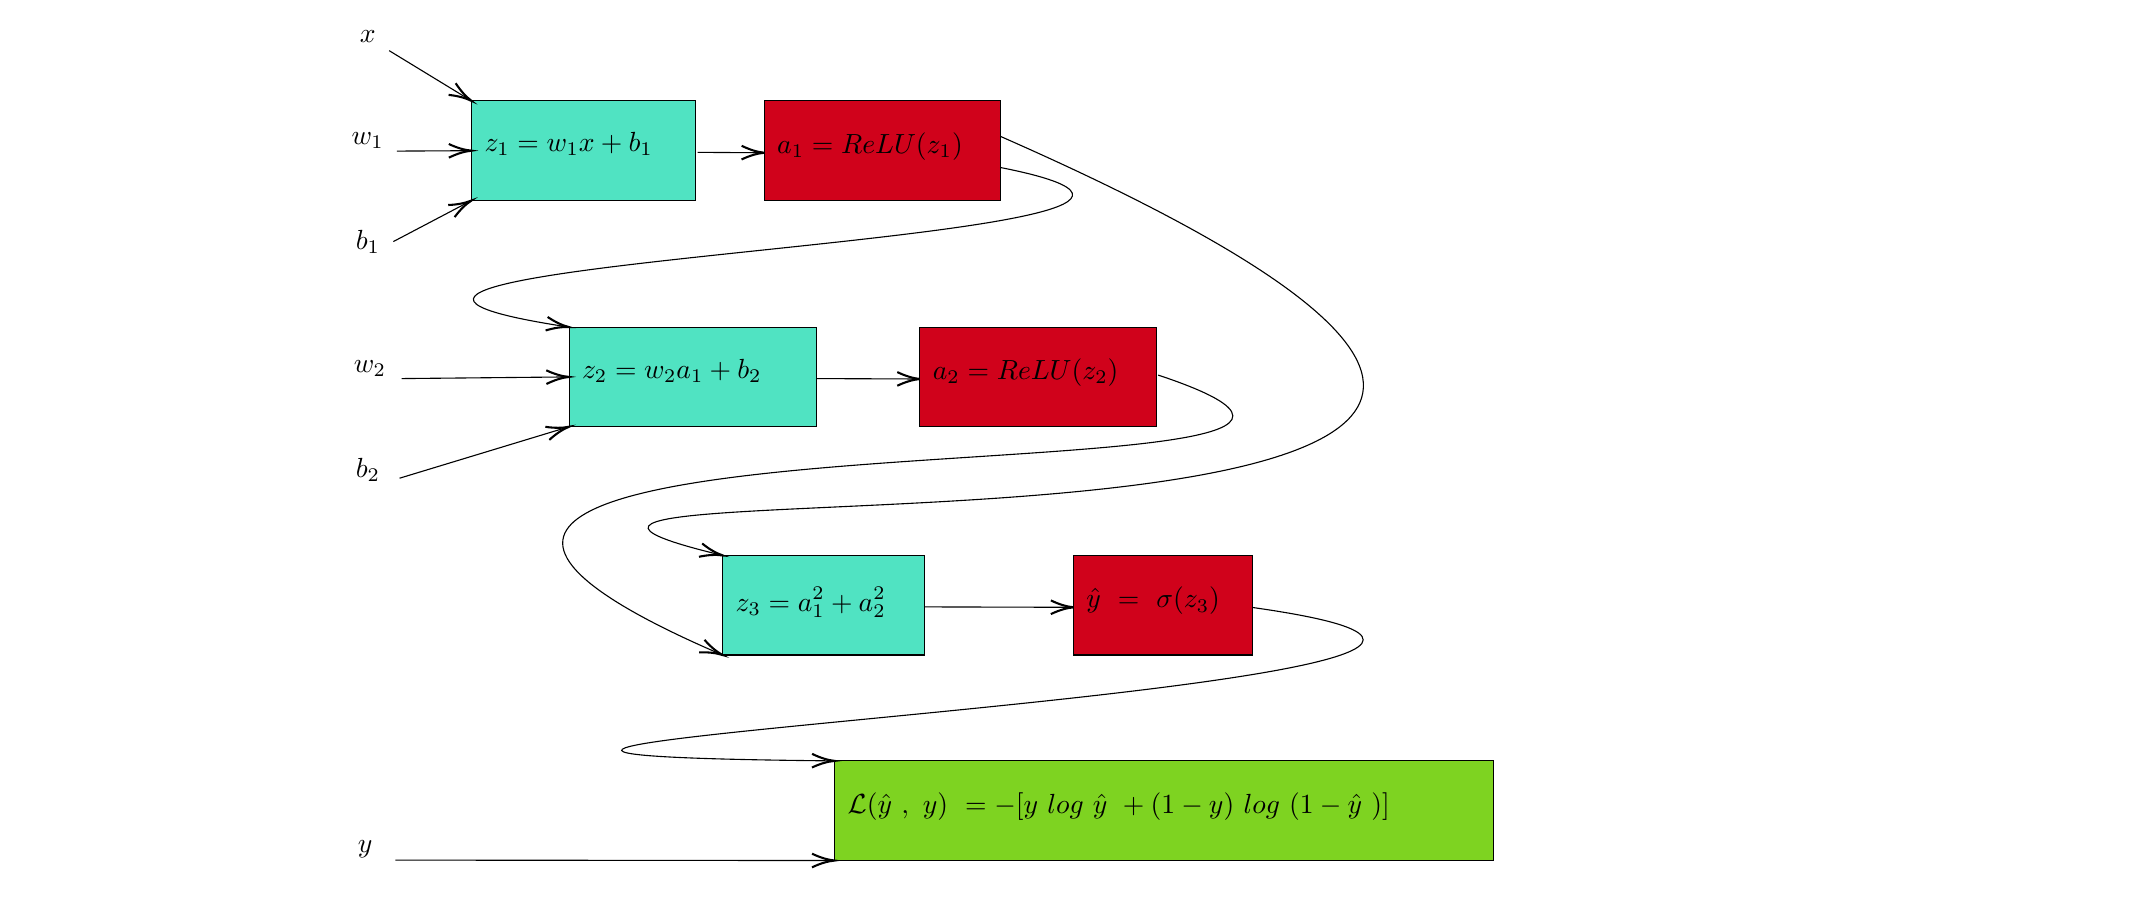
\begin{tikzpicture}[x=0.75pt,y=0.75pt,yscale=-1,xscale=1]
%uncomment if require: \path (0,433); %set diagram left start at 0, and has height of 433

%Shape: Rectangle [id:dp26082320028943795] 
\draw  [fill={rgb, 255:red, 80; green, 227; blue, 194 }  ,fill opacity=1 ] (62,46) -- (170.07,46) -- (170.07,94) -- (62,94) -- cycle ;
%Straight Lines [id:da5321728940522126] 
\draw    (22.33,21.8) -- (60.29,44.96) ;
\draw [shift={(62,46)}, rotate = 211.39] [color={rgb, 255:red, 0; green, 0; blue, 0 }  ][line width=0.75]    (10.93,-3.29) .. controls (6.95,-1.4) and (3.31,-0.3) .. (0,0) .. controls (3.31,0.3) and (6.95,1.4) .. (10.93,3.29)   ;
%Straight Lines [id:da8722522064456113] 
\draw    (26.07,70.2) -- (60,70.01) ;
\draw [shift={(62,70)}, rotate = 179.68] [color={rgb, 255:red, 0; green, 0; blue, 0 }  ][line width=0.75]    (10.93,-3.29) .. controls (6.95,-1.4) and (3.31,-0.3) .. (0,0) .. controls (3.31,0.3) and (6.95,1.4) .. (10.93,3.29)   ;
%Straight Lines [id:da4977170317452869] 
\draw    (24.33,113.8) -- (60.23,94.93) ;
\draw [shift={(62,94)}, rotate = 152.27] [color={rgb, 255:red, 0; green, 0; blue, 0 }  ][line width=0.75]    (10.93,-3.29) .. controls (6.95,-1.4) and (3.31,-0.3) .. (0,0) .. controls (3.31,0.3) and (6.95,1.4) .. (10.93,3.29)   ;
%Straight Lines [id:da9786960106080183] 
\draw    (171,70.8) -- (201.07,70.99) ;
\draw [shift={(203.07,71)}, rotate = 180.36] [color={rgb, 255:red, 0; green, 0; blue, 0 }  ][line width=0.75]    (10.93,-3.29) .. controls (6.95,-1.4) and (3.31,-0.3) .. (0,0) .. controls (3.31,0.3) and (6.95,1.4) .. (10.93,3.29)   ;
%Shape: Rectangle [id:dp4699732294865028] 
\draw  [fill={rgb, 255:red, 208; green, 2; blue, 27 }  ,fill opacity=1 ] (203,46) -- (317.07,46) -- (317.07,94) -- (203,94) -- cycle ;
%Shape: Rectangle [id:dp7233773663060797] 
\draw  [fill={rgb, 255:red, 80; green, 227; blue, 194 }  ,fill opacity=1 ] (109,155) -- (228.33,155) -- (228.33,203) -- (109,203) -- cycle ;
%Straight Lines [id:da5907930980218636] 
\draw    (28.33,179.8) -- (107,179.02) ;
\draw [shift={(109,179)}, rotate = 179.43] [color={rgb, 255:red, 0; green, 0; blue, 0 }  ][line width=0.75]    (10.93,-3.29) .. controls (6.95,-1.4) and (3.31,-0.3) .. (0,0) .. controls (3.31,0.3) and (6.95,1.4) .. (10.93,3.29)   ;
%Straight Lines [id:da5935250653594418] 
\draw    (27.33,227.8) -- (107.09,203.58) ;
\draw [shift={(109,203)}, rotate = 163.11] [color={rgb, 255:red, 0; green, 0; blue, 0 }  ][line width=0.75]    (10.93,-3.29) .. controls (6.95,-1.4) and (3.31,-0.3) .. (0,0) .. controls (3.31,0.3) and (6.95,1.4) .. (10.93,3.29)   ;
%Straight Lines [id:da4807719277385877] 
\draw    (228.33,179.8) -- (276.07,179.99) ;
\draw [shift={(278.07,180)}, rotate = 180.23] [color={rgb, 255:red, 0; green, 0; blue, 0 }  ][line width=0.75]    (10.93,-3.29) .. controls (6.95,-1.4) and (3.31,-0.3) .. (0,0) .. controls (3.31,0.3) and (6.95,1.4) .. (10.93,3.29)   ;
%Shape: Rectangle [id:dp004733566676465184] 
\draw  [fill={rgb, 255:red, 208; green, 2; blue, 27 }  ,fill opacity=1 ] (278,155) -- (392.07,155) -- (392.07,203) -- (278,203) -- cycle ;
%Curve Lines [id:da43051210766963555] 
\draw    (316.83,78.1) .. controls (498.83,114.1) and (-103.67,122.8) .. (109,155) ;
\draw [shift={(109,155)}, rotate = 188.61] [color={rgb, 255:red, 0; green, 0; blue, 0 }  ][line width=0.75]    (10.93,-3.29) .. controls (6.95,-1.4) and (3.31,-0.3) .. (0,0) .. controls (3.31,0.3) and (6.95,1.4) .. (10.93,3.29)   ;
%Shape: Rectangle [id:dp7844392260191501] 
\draw  [fill={rgb, 255:red, 80; green, 227; blue, 194 }  ,fill opacity=1 ] (183,265) -- (280.33,265) -- (280.33,313) -- (183,313) -- cycle ;
%Straight Lines [id:da7438844634576284] 
\draw    (280.33,289.8) -- (350.07,289.99) ;
\draw [shift={(352.07,290)}, rotate = 180.16] [color={rgb, 255:red, 0; green, 0; blue, 0 }  ][line width=0.75]    (10.93,-3.29) .. controls (6.95,-1.4) and (3.31,-0.3) .. (0,0) .. controls (3.31,0.3) and (6.95,1.4) .. (10.93,3.29)   ;
%Shape: Rectangle [id:dp06514973867064988] 
\draw  [fill={rgb, 255:red, 208; green, 2; blue, 27 }  ,fill opacity=1 ] (352,265) -- (438.33,265) -- (438.33,313) -- (352,313) -- cycle ;
%Curve Lines [id:da5234327252277915] 
\draw    (316.83,63.1) .. controls (853.83,299.1) and (-37.87,212.1) .. (183,265) ;
\draw [shift={(183,265)}, rotate = 193.47] [color={rgb, 255:red, 0; green, 0; blue, 0 }  ][line width=0.75]    (10.93,-3.29) .. controls (6.95,-1.4) and (3.31,-0.3) .. (0,0) .. controls (3.31,0.3) and (6.95,1.4) .. (10.93,3.29)   ;
%Curve Lines [id:da12663621077553533] 
\draw    (392.83,178.1) .. controls (593.17,244.9) and (-122.67,181.8) .. (183,313) ;
\draw [shift={(183,313)}, rotate = 203.23] [color={rgb, 255:red, 0; green, 0; blue, 0 }  ][line width=0.75]    (10.93,-3.29) .. controls (6.95,-1.4) and (3.31,-0.3) .. (0,0) .. controls (3.31,0.3) and (6.95,1.4) .. (10.93,3.29)   ;
%Shape: Rectangle [id:dp1997427400696722] 
\draw  [fill={rgb, 255:red, 126; green, 211; blue, 33 }  ,fill opacity=1 ] (237,364) -- (554.43,364) -- (554.43,412) -- (237,412) -- cycle ;
%Straight Lines [id:da05813852175573886] 
\draw    (25.33,411.8) -- (235,412) ;
\draw [shift={(237,412)}, rotate = 180.05] [color={rgb, 255:red, 0; green, 0; blue, 0 }  ][line width=0.75]    (10.93,-3.29) .. controls (6.95,-1.4) and (3.31,-0.3) .. (0,0) .. controls (3.31,0.3) and (6.95,1.4) .. (10.93,3.29)   ;
%Curve Lines [id:da6379195786923225] 
\draw    (438.43,290.1) .. controls (707.43,328.1) and (-151.57,360.1) .. (237,364) ;
\draw [shift={(237,364)}, rotate = 180.58] [color={rgb, 255:red, 0; green, 0; blue, 0 }  ][line width=0.75]    (10.93,-3.29) .. controls (6.95,-1.4) and (3.31,-0.3) .. (0,0) .. controls (3.31,0.3) and (6.95,1.4) .. (10.93,3.29)   ;

% Text Node
\draw (67,60) node [anchor=north west][inner sep=0.75pt]   [align=left] {$\displaystyle z_{1} =w_{1} x+b_{1}$};
% Text Node
\draw (7,11) node [anchor=north west][inner sep=0.75pt]   [align=left] {$\displaystyle x$};
% Text Node
\draw (3,60) node [anchor=north west][inner sep=0.75pt]   [align=left] {$\displaystyle w_{1}$};
% Text Node
\draw (5,107) node [anchor=north west][inner sep=0.75pt]   [align=left] {$\displaystyle b_{1}$};
% Text Node
\draw (208,60) node [anchor=north west][inner sep=0.75pt]   [align=left] {$\displaystyle a_{1} =ReLU( z_{1})$};
% Text Node
\draw (114,169) node [anchor=north west][inner sep=0.75pt]   [align=left] {$\displaystyle z_{2} =w_{2} a_{1} +b_{2}$};
% Text Node
\draw (4,170) node [anchor=north west][inner sep=0.75pt]   [align=left] {$\displaystyle w_{2}$};
% Text Node
\draw (5,217) node [anchor=north west][inner sep=0.75pt]   [align=left] {$\displaystyle b_{2}$};
% Text Node
\draw (283,169) node [anchor=north west][inner sep=0.75pt]   [align=left] {$\displaystyle a_{2} =ReLU( z_{2})$};
% Text Node
\draw (188,279) node [anchor=north west][inner sep=0.75pt]   [align=left] {$\displaystyle z_{3} =a_{1}^{2} +a_{2}^{2}$};
% Text Node
\draw (357,279) node [anchor=north west][inner sep=0.75pt]   [align=left] {$\displaystyle \hat{y} \ =\ \sigma ( z_{3})$};
% Text Node
\draw (242,378) node [anchor=north west][inner sep=0.75pt]   [align=left] {$\displaystyle \mathcal{L}(\hat{y} \ ,\ y) \ =-[ y\ log\ \hat{y} \ +( 1-y) \ log\ ( 1-\hat{y} \ )] \ $};
% Text Node
\draw (6,401) node [anchor=north west][inner sep=0.75pt]   [align=left] {$\displaystyle y$};


\end{tikzpicture}

\end{latin}


\subsection{ب}
\begin{latin}
$
\frac{\partial L}{\partial a_1} =
\frac{\partial L}{\partial \hat{y}} \times
\frac{\partial \hat{y}}{\partial z_3} \times
\frac{\partial z_3}{\partial a_1} =
\left(\frac{-y}{\hat{y}} + \frac{1-y}{1-\hat{y}}\right) \times
\hat{y}\left( 1-\hat{y} \right) \times
2a_1 =
\left( \hat{y} - y \right)2a_1
$
\\
\\
$
\frac{\partial L}{\partial a_2} =
\frac{\partial L}{\partial \hat{y}} \times
\frac{\partial \hat{y}}{\partial z_3} \times
\frac{\partial z_3}{\partial a_2} =
\left(\frac{-y}{\hat{y}} + \frac{1-y}{1-\hat{y}}\right) \times
\hat{y}\left( 1-\hat{y} \right) \times
2a_2 =
\left( \hat{y} - y \right)2a_2
$
\\
\\
$
\frac{\partial L}{\partial w_1} =
\frac{\partial L}{\partial \hat{y}} \times
\frac{\partial \hat{y}}{\partial z_3} \times
\left(
\frac{\partial z_3}{\partial a_1} \times \frac{\partial a_1}{\partial z_1} \times \frac{\partial z_1}{\partial w_1}            +
\frac{\partial z_3}{\partial a_2} \times \frac{\partial a_2}{\partial z_2} \times \frac{\partial z_2}{\partial a_1} \times \frac{\partial a_1}{\partial z_1} \times \frac{\partial z_1}{\partial w_1}
\right)
\\=
\frac{\partial L}{\partial a_1} \times \frac{\partial a_1}{\partial z_1} \times \frac{\partial z_1}{\partial w_1}
+
\frac{\partial L}{\partial a_2} \times \frac{\partial a_2}{\partial z_2} \times \frac{\partial z_2}{\partial a_1} \times \frac{\partial a_1}{\partial z_1} \times \frac{\partial z_1}{\partial w_1}
\\=
\left( \hat{y} - y \right)2a_1 \times a_1\left( 1 - a_1 \right) \times x
+
\left( \hat{y} - y \right)2a_2 \times a_2\left( 1 - a_2 \right) \times w_2 \times a_1\left( 1 - a_1 \right) \times x
\\=
2\left( \hat{y} - y \right)a_1\left( 1 - a_1 \right)x\left[ a_1 + a_2 ^ 2\left( 1 - a_2 \right) w_2 \right]
$
\\
\\
$
\frac{\partial L}{\partial w_2} =
\frac{\partial L}{\partial \hat{y}} \times
\frac{\partial \hat{y}}{\partial z_3} \times
\frac{\partial z_3}{\partial a_2} \times
\frac{\partial a_2}{\partial z_2} \times
\frac{\partial z_2}{\partial w_2} 
\\=
\frac{\partial L}{\partial a_2} \times
\frac{\partial a_2}{\partial z_2} \times
\frac{\partial z_2}{\partial w_2} =
\left( \hat{y} - y \right)2a_2 \times a_2\left( 1 - a_2 \right) \times a_1
$
\end{latin}


%\begin{enumerate}
%	\item \lr{Bob} لیستی از الگوریتم‌هایی که از آن‌ها پشتیبانی می‌کند را به همراه \lr{nonce} به \lr{Alice} می‌فرستد.
%	\item \lr{Alice} بین لیست الگوریتم‌های پیشنهادی یکی را انتخاب می‌کند و آن را به همراه \lr{certificate} و \lr{nonce} می‌فرستد.
%	\item \lr{Bob} \lr{certificate} را اعتبارسنجی می‌کند، \lr{public key}ِ \lr{Alice} را استخراج می‌کند، \lr{pre\_master\_secret} را تولید می‌کند، با \lr{public key}ِ \lr{Alice} آن را رمز می‌کند و برای \lr{Alice} می‌فرستد.
%	\item \lr{Bob} و \lr{Alice} به طور مستقل رمز و کلیدهای \lr{MAC} را از \lr{pre\_master\_secret} و \lr{nonce}ها محاسبه می‌کنند.
%	\item \lr{Bob} یک \lr{MAC} از همه‌ی پیام‌های \lr{handshake} می‌فرستد.
%	\item \lr{Alice} یک \lr{MAC} از همه‌ی پیام‌های \lr{handshake} می‌فرستد.
%\end{enumerate}




%%%%%%%%%%%%%%%%%%%%%%%%%%%%%%%%%%%
%%%%%%%%%%%%%%%%%%%%%%%%%%%%%%%%%%%
%%%%%%%%%%%%%%%%%%%%%%%%%%%%%%%%%%%



\section*{منابع}
\renewcommand{\section}[2]{}%
\begin{thebibliography}{99} % assumes less than 100 references
%چنانچه مرجع فارسی نیز داشته باشید باید دستور فوق را فعال کنید و مراجع فارسی خود را بعد از این دستور وارد کنید


\begin{LTRitems}

\resetlatinfont

\bibitem{b1} https://www.shiksha.com/online-courses/articles/relu-and-sigmoid-activation-function/
\bibitem{b1} https://medium.com/@amanatulla1606/vanishing-gradient-problem-in-deep-learning-understanding-intuition-and-solutions-da90ef4ecb54
\bibitem{b1} https://en.wikipedia.org/wiki/Rectifier\_(neural\_networks)
\bibitem{b1} https://wandb.ai/ayush-thakur/dl-question-bank/reports/ReLU-vs-Sigmoid-Function-in-Deep-Neural-Networks--VmlldzoyMDk0MzI
\bibitem{b1} https://medium.com/swlh/why-are-neural-nets-non-linear-a46756c2d67f
\end{LTRitems}

\end{thebibliography}


\end{document}
